\documentclass{article}
\usepackage{geometry}
\usepackage{tikz}
\usepackage[most]{tcolorbox}
\usepackage{mathabx}
\usepackage{booktabs}

% https://tex.stackexchange.com/questions/198658/
\makeatletter
\newcommand\incircbin
{\mathpalette\@incircbin}
\newcommand\@incircbin[2]
{\mathbin{\ooalign{\hidewidth$#1#2$\hidewidth\crcr$#1\ovoid$}}}
\newcommand{\ocol}{\incircbin{:}}
\makeatother

\geometry{a4paper, total={170mm, 257mm}, left=20mm}
\linespread{1.8}

\tcbset{on line, box align=base,
    sharp corners=northwest,sharp corners=southeast,
    boxsep=4pt, left=0pt,right=0pt,top=0pt,bottom=0pt,
    grow to left by=5pt,
    colframe=white
}
\newcommand{\splitbox}[3]{
    \tcbox[enhanced, interior code={%
        \path[fill=#1,rounded corners=5px] (interior.north west) |- (interior.south east);
        \path[fill=#2,rounded corners=5px] (interior.south east) |- (interior.north west);
    }]{#3}
}

\colorlet{instr-arg}{red!30!green!20}
\colorlet{instr-jsp}{blue!90!green!20}
\colorlet{instr-u32}{orange!90!black!20}

\begin{document}
\pagestyle{empty}
\begin{minipage}{0.3\textwidth}
\begin{tabular}{rll}
    \texttt{02} & $\ominus$ & \texttt{pop}                                       \\
    \texttt{01} & $\oplus$  & \tcbox[colback=instr-arg]{\texttt{push + a}}       \\
    \texttt{04} & $\oplus$  & \texttt{divine}                                    \\
    \texttt{03} & $\oplus$  & \tcbox[colback=instr-arg]{\texttt{dup + i}}        \\
    \texttt{05} &           & \tcbox[colback=instr-arg]{\texttt{swap + i}}       \\
    \texttt{06} & $\ovoid$  & \texttt{nop}                                       \\
    \texttt{08} & $\ominus$ & \tcbox[colback=instr-jsp]{\texttt{skiz}}           \\
    \texttt{07} & $\ovoid$  & \splitbox{instr-jsp}{instr-arg}{\texttt{call + d}} \\
    \texttt{10} & $\ovoid$  & \tcbox[colback=instr-jsp]{\texttt{return}}         \\
    \texttt{12} & $\ovoid$  & \tcbox[colback=instr-jsp]{\texttt{recurse}}        \\
    \texttt{14} & $\ominus$ & \texttt{assert}                                    \\
    \texttt{00} & $\ovoid$  & \texttt{halt}                                      \\
    \texttt{16} & $\odot$   & \texttt{read\_mem}                                 \\
    \texttt{18} & $\ovoid$  & \texttt{write\_mem}                                \\
    \texttt{20} &           & \texttt{hash}                                      \\
    \texttt{22} &           & \texttt{divine\_sibling}                           \\
    \texttt{24} & $\ovoid$  & \texttt{assert\_vector}                            \\
    \texttt{26} & $\ocol$   & \texttt{add}                                       \\
    \texttt{28} & $\ocol$   & \texttt{mul}                                       \\
    \texttt{30} & $\odot$   & \texttt{invert}                                    \\
    \texttt{32} &           & \texttt{split}                                     \\
    \texttt{34} & $\ocol$   & \texttt{eq}                                        \\
    \texttt{36} & $\ocol$   & \tcbox[colback=instr-u32]{\texttt{lt}}             \\
    \texttt{38} & $\ocol$   & \tcbox[colback=instr-u32]{\texttt{and}}            \\
    \texttt{40} & $\ocol$   & \tcbox[colback=instr-u32]{\texttt{xor}}            \\
    \texttt{42} & $\odot$   & \tcbox[colback=instr-u32]{\texttt{reverse}}        \\
    \texttt{44} &           & \tcbox[colback=instr-u32]{\texttt{div}}            \\
    \texttt{46} &           & \texttt{xxadd}                                     \\
    \texttt{48} &           & \texttt{xxmul}                                     \\
    \texttt{50} &           & \texttt{xinv}                                      \\
    \texttt{52} &           & \texttt{xbmul}                                     \\
    \texttt{54} & $\oplus$  & \texttt{read\_io}                                  \\
    \texttt{56} & $\ominus$ & \texttt{write\_io}
\end{tabular}
\end{minipage}\hfill%
\begin{minipage}[][0.84\textheight][s]{0.6\textwidth}
    \hfill
    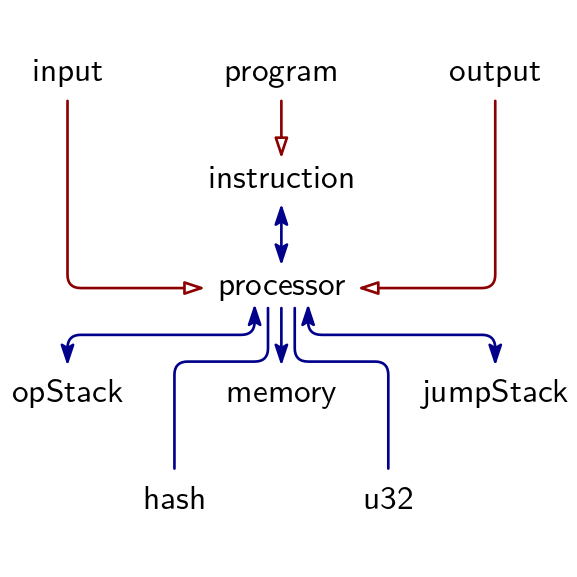
\includegraphics[keepaspectratio,width=0.9\textwidth]{img/aet-relations.pdf}
    \vfill

    \hfill
    \begin{tabular}{lrrr}
        \toprule
                    & base & ext & full \\ \midrule
        Program     &    2 &   2 &    4 \\
        Instruction &    3 &   4 &    7 \\
        Processor   &   36 &  24 &   60 \\
        OpStack     &    4 &   2 &    6 \\
        RAM         &    4 &   2 &    6 \\
        JumpStack   &    5 &   2 &    7 \\
        Hash        &   17 &   4 &   21 \\
        U32         &    7 &  10 &   17 \\ \bottomrule\bottomrule
                    &   78 &  50 &  128
    \end{tabular}
\end{minipage}
\end{document}
